%To compile as handout, use
%pdflatex "\def\ishandout{1} \input{filename.tex}"
%Defaults to non-handout mode (with slide reveals)
\ifdefined\ishandout
  \documentclass[handout]{beamer}
\else
  \documentclass{beamer}
\fi
 
\usepackage{econ103slides} 

\date{Lecture \# 9}
\begin{document} 

%%%%%%%%%%%%%%%%%%%%%%%%%%%%%%%%%%%%%%%%

\begin{frame}[plain]
	\titlepage 
	

\end{frame} 

%%%%%%%%%%%%%%%%%%%%%%%%%%%%%%%%%%%%%%%%

\begin{frame}
\centering \Huge Discrete RVs -- Part II

\end{frame}



%%%%%%%%%%%%%%%%%%%%%%%%%%%%%%%%%%%%%%%%

\begin{frame}
\frametitle{Linearity of Expectation}
\framesubtitle{Holds for Continuous RVs as well, but proof is different.}
Let $X$ be a RV and $a,b$ be constants. Then:
	$$E[a + bX] = a + bE[X]$$
\vspace{2em}
\begin{alertblock}{This is one of the most important facts in the course: the special case in which $E[g(X)] = g(E[X])$ is $g = a+bX$.}
\end{alertblock}
\end{frame}
%%%%%%%%%%%%%%%%%%%%%%%%%%%%%%%%%%%%%%%%
\begin{frame}
\frametitle{Proof: Linearity of Expectation For Discrete RV}

\begin{eqnarray*}
	E[a + bX] &=& \pause \sum_{\mbox{all } x}  (a + bx) p(x)\\ \\
	 &=&\pause  \sum_{\mbox{all } x} p(x) \cdot a + \sum_{\mbox{all } x}p(x) \cdot bx\\ \\
	&=& \pause a\sum_{\mbox{all } x} p(x) + b\sum_{\mbox{all } x} x \cdot p(x) \\ \\
	&=& \pause a + b E[X]
\end{eqnarray*}


\end{frame}
%%%%%%%%%%%%%%%%%%%%%%%%%%%%%%%%%%%%%%%%

\begin{frame}
\frametitle{Variance and Standard Deviation of a RV}
\framesubtitle{The Defs are the same for continuous RVs, but the method of calculating will differ.}

\begin{block}{Variance (Var)}
	$$\sigma^2 = Var(X) = E\left[ (X - \mu)^2\right] = E\left[ (X - E[X])^2\right]$$
\end{block}


\begin{block}{Standard Deviation (SD)}
$$\sigma = \sqrt{\sigma^2} = SD(X)$$
\end{block}


\end{frame}
%%%%%%%%%%%%%%%%%%%%%%%%%%%%%%%%%%%%%%%%
\begin{frame}
\frametitle{Key Point}

\alert{Variance and std.\ dev.\ are \emph{expectations of functions of a RV}} 

\vspace{1em}

It follows that: 
\begin{enumerate}
\item Variance and SD are constants
\item To derive facts about them you can use the facts you know about expected value
\end{enumerate}
\end{frame}
%%%%%%%%%%%%%%%%%%%%%%%%%%%%%%%%%%%%%%%%
\begin{frame}
\frametitle{How To Calculate Variance for Discrete RV?}
\framesubtitle{Remember: it's just a function of $X$!}


Recall that	$\displaystyle \mu = E[X] = \sum_{\mbox{all } x} xp(x)$


\vspace{3em}

$$Var(X) = E\left[ (X - \mu)^2 \right] =\sum_{\mbox{all } x} (x - \mu)^2 p(x)$$


\end{frame}
%%%%%%%%%%%%%%%%%%%%%%%%%%%%%%%%%%%%%%%%
\begin{frame}
\frametitle{Shortcut Formula For Variance}

This is \emph{not} the definition, it's a shortcut for doing calculations:
\begin{eqnarray*}
	Var(X) = E\left[ (X - \mu)^2 \right] = E[X^2] - \left(E[X]\right)^2
\end{eqnarray*}

\alert{We'll prove this in an upcoming lecture.}

\end{frame}

%%%%%%%%%%%%%%%%%%%%%%%%%%%%%%%%%%%%%%%%


\begin{frame}
\frametitle{Variance of Bernoulli RV -- via the Shortcut Formula}

\begin{block}{Step 1 -- $E[X]$} 
$\mu = E[X] = \displaystyle \sum_{x \in \{0,1\}} p(x) \cdot x = (1-p) \cdot 0 + p \cdot 1 = p$
\end{block}

\pause

\begin{block}{Step 2 -- $E[X^2]$} 
\begin{eqnarray*}
	E[X^2] = \sum_{x \in \{0,1\}} x^2 p(x) = 0^2 (1-p) + 1^2 p = p
\end{eqnarray*}
\end{block}

\pause

\begin{block}{Step 3 -- Combine with Shortcut Formula} 
\begin{eqnarray*}
	\sigma^2 = Var[X] = E[X^2] - \left(E[X]\right)^2 = \ p - p^2 =  p(1-p)
\end{eqnarray*}
\end{block}


\end{frame}
%%%%%%%%%%%%%%%%%%%%%%%%%%%%%%%%%%%%%%%%



\begin{frame}
\frametitle{Variance of Bernoulli RV -- Without Shortcut}

\alert{You will fill in the missing steps on Problem Set 5.}

\begin{eqnarray*}
	\sigma^2 &=& Var(X) = \sum_{x \in \{0,1\}} (x - \mu)^2 p(x)\\
	 &=& \sum_{x \in \{0,1\}} (x - p)^2 p(x)\\
	 &\vdots &\\ 
	 &=&p(1-p)
\end{eqnarray*}

%%%%%%%%%%%%%%%%%%%%%%%%%%%%%%%%%%%%%%%%


\end{frame}

\begin{frame}
\frametitle{Variance of a Linear Function  \hfill 
\includegraphics[scale = 0.05]{./images/clicker} }
Suppose $X$ is a random variable with $Var(X) = \sigma^2$ and $a,b$ are constants. What is $Var(a + bX)$? 
\begin{enumerate}[(a)]
	\item $\sigma^2$
	\item $a + \sigma^2$
	\item $b \sigma^2$
	\item $a + b \sigma^2$
	\item $b^2 \sigma^2$
\end{enumerate}

\end{frame}
%%%%%%%%%%%%%%%%%%%%%%%%%%%%%%%%%%%%%%%%
\begin{frame}
	\frametitle{Variance and SD are \emph{NOT} Linear}

\begin{eqnarray*}
Var(a + bX) &= &b^2 \sigma^2 \\\\
	SD(a + bX)&=& |b| \sigma
\end{eqnarray*}

\vspace{2em}
\begin{block}{These should look familiar from the related results for sample variance and std.\ dev. that you worked out on an earlier problem set.}

\end{block}

\end{frame}
%%%%%%%%%%%%%%%%%%%%%%%%%%%%%%%%%%%%%%%%
\begin{frame}
\frametitle{Variance of a Linear Transformation}

\begin{eqnarray*}
 Var(a + bX) &=& E\left[\left\{(a+bX) - E(a+bX)\right\}^2 \right] \\ \pause
 	&=& E\left[\left\{(a+bX) - (a+bE[X])\right\}^2 \right] \\ \pause
 	&=&E\left[\left(bX - bE[X]\right)^2 \right] \\ \pause
 	&=&E[b^2 (X - E[X])^2]\\ \pause
 	&=& b^2 E[(X-E[X])^2]\\ \pause
 	&=& b^2 Var(X) = b^2 \sigma^2
\end{eqnarray*}
\alert{The key point here is that variance is defined in terms of expectation and expectation is linear.}

\end{frame}
%%%%%%%%%%%%%%%%%%%%%%%%%%%%%%%%%%%%%%%%
\begin{frame}
	\begin{center}
		\Huge Binomial Random Variable	\\
		\large What we get if we sum a bunch of indep.\ Bernoulli RVs
	\end{center}
\end{frame}

%%%%%%%%%%%%%%%%%%%%%%%%%%%%%%%%%%%%%%%%

\begin{frame}
\frametitle{
\includegraphics[scale = 0.05]{./images/clicker} }
\begin{block}{Question}
Suppose we flip a fair coin 3 times. What is the probability that we get exactly 2 heads?
\end{block}

\pause

\begin{block}{Answer}
Three basic outcomes make up this event: $\{HHT, HTH, THH\}$. \pause Each of these has probability $1/8 = 1/2 \times 1/2 \times 1/2$ so, since basic outcomes are mutually exclusive we sum to get \alert{$3/8 = 0.375$}
\end{block}

\end{frame}
%%%%%%%%%%%%%%%%%%%%%%%%%%%%%%%%%%%%%%%%
\begin{frame}
\frametitle{A More Complicated Example}
\begin{block}{Question}
Suppose we flip an \emph{unfair} coin 3 times, where the probability of heads is 1/3. What is the probability that we get exactly 2 heads?
\end{block}



\begin{block}{Answer}
The basic outcomes of the experiment are no longer equally likely, but those with exactly two heads \emph{\alert{remain so}} 
	\begin{eqnarray*}
	 P(HHT) &=&  (1/3)^2 (1 - 1/3) =  2/27\\ 
	 P(THH) &=&2/27\\ 
	 P(HTH) &=&2/27 
	\end{eqnarray*}
	Summing gives \alert{$2/9 \approx 0.22$}
\end{block}
\end{frame}
%%%%%%%%%%%%%%%%%%%%%%%%%%%%%%%%%%%%%%%%
\begin{frame}
\frametitle{Starting to see a pattern?}

Suppose we flip an unfair coin \emph{4} times, where the probability of heads is 1/3. What is the probability that we get exactly 2 heads?

\vspace{2em}



\begin{columns}
\column{0.35\textwidth}
\begin{tabular}{cc}
HHTT&TTHH\\
HTHT&THTH\\
HTTH&THHT
\end{tabular}

\column{0.55\textwidth}
\alert{Six equally likely, mutually exclusive basic outcomes make up this event:}
$${4\choose 2}(1/3)^2(2/3)^2$$
\end{columns}

\end{frame}

%%%%%%%%%%%%%%%%%%%%%%%%%%%%%%%%%%%%%%%%

\begin{frame}
\frametitle{Binomial Random Variable}
Let $X = $ the sum of $n$ independent Bernoulli trials, each with probability of success $p$.  \alert{Then we say that:
		$X \sim \mbox{Binomial}(n,p)$} 

\vspace{2em}
\begin{block}{Parameters}
$p =$ probability of ``success,'' $n=$ \# of trials
\end{block}
\begin{block}{Support} 
$\{0, 1, 2, \hdots, n\}$ 
\end{block}
\begin{block}{Probability Mass Function (pmf)} 
$$p(x) = {n \choose x} p^x (1-p)^{n-x}$$ 
\end{block}
\end{frame}
%%%%%%%%%%%%%%%%%%%%%%%%%%%%%%%%%%%%%%%%

\begin{frame}
	\frametitle{\href{http://glimmer.rstudio.com/fditraglia/binom_cdf/}{http://glimmer.rstudio.com/fditraglia/binom\_cdf/}}
\framesubtitle{Try playing around with all three sliders. If you set the second to 1 you get a Bernoulli.}

\begin{figure}
	\fbox{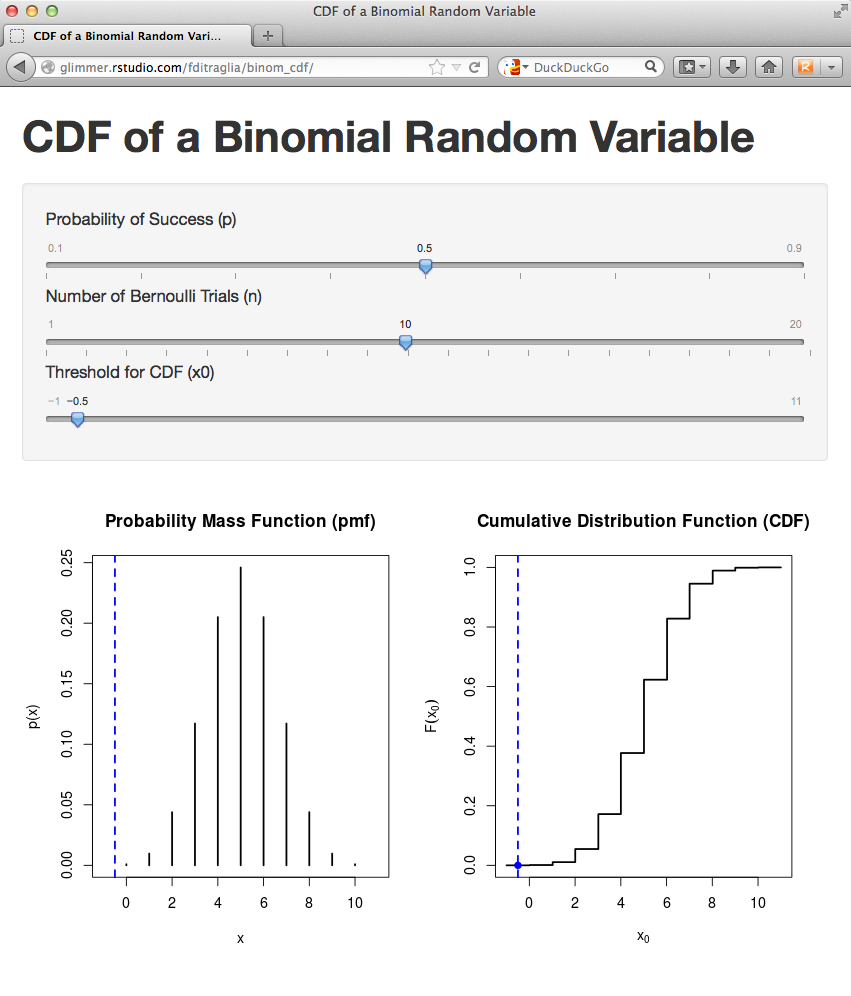
\includegraphics[scale = 0.2]{./images/binom_cdf_screenshot2}}
\end{figure}

\end{frame}

%%%%%%%%%%%%%%%%%%%%%%%%%%%%%%%%%%%%%%%%



\begin{frame}
\frametitle{Don't forget this!}
 \large A Binomial Random Variable counts up the \emph{total} number of successes (ones) in $n$ independent Bernoulli trials, each with probability of success $p$.


\vspace{5em}
\alert{We'll learn more about the Binomial RV in the coming lectures...}
\end{frame}
%%%%%%%%%%%%%%%%%%%%%%%%%%%%%%%%%%%%%%%%

\begin{frame}
	\frametitle{\href{http://fditraglia.github.com/Econ103Public/Rtutorials/Bernoulli_Binomial.html}{\small http://fditraglia.github.com/Econ103Public/Rtutorials/Bernoulli\_Binomial.html}}

\framesubtitle{Source Code on my \href{https://github.com/fditraglia/Econ103Public/blob/master/Rtutorials/Bernoulli_Binomial.R}{\fbox{Github Page}}}



\begin{figure}
	\fbox{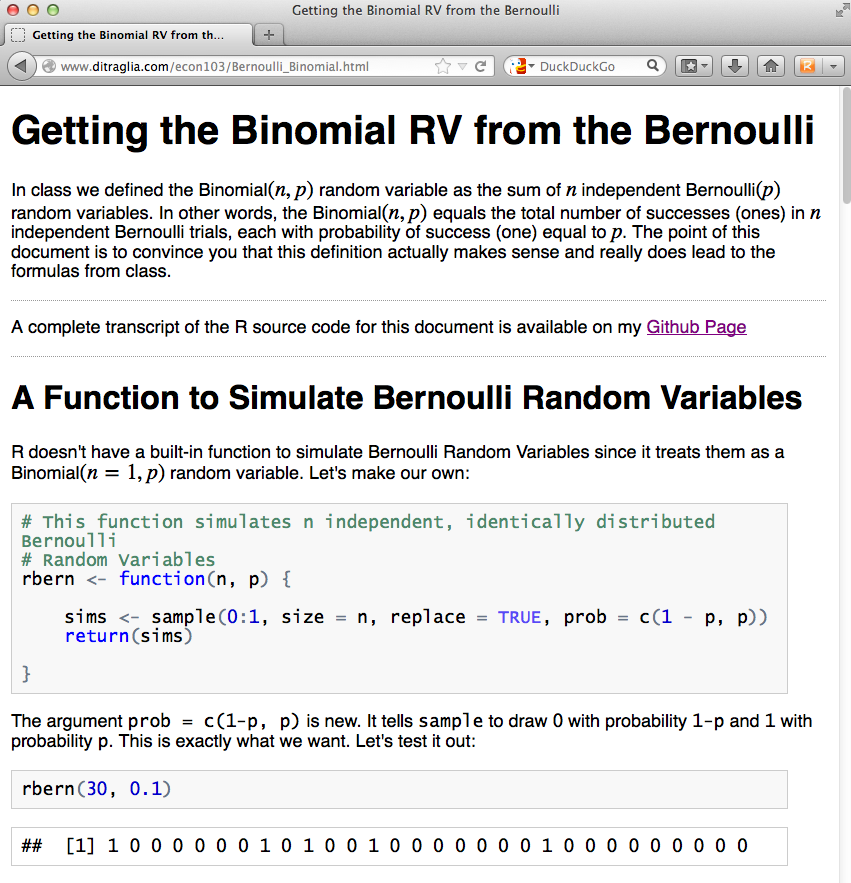
\includegraphics[scale = 0.2]{./images/binom_bernoulli_sim_screenshot}}
\end{figure}

\end{frame}

%%%%%%%%%%%%%%%%%%%%%%%%%%%%%%%%%%%%%%%%


\end{document}
